\section{Fundamento teórico}

Para comenzar se deben establecer unos parámetros para con la pala, ya que lo más básico de este trabajo empieza por determinar los efectos que produce la torsión en nuestra obtención de energía.

Es por ello que se determina que la pala de la turbina eólica es un trapecio cuya representación simplificada la vemos en la Figura \ref{fig:pala_simp}

\begin{figure}[H]
    \centering
    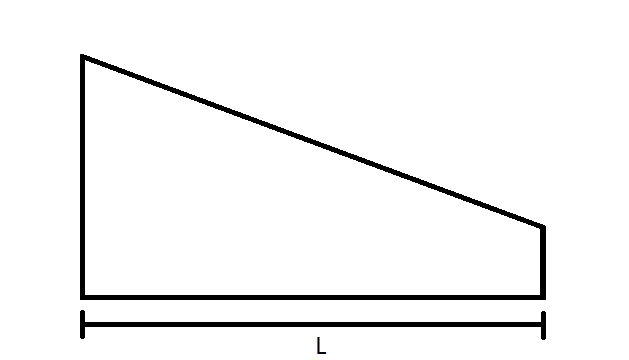
\includegraphics[width=0.7\textwidth]{images/pala turbina paint.png}
    \caption{Representación de una pala de turbina eólica}
    \label{fig:pala_simp}
\end{figure}


Lo siguiente que se debe hacer es dividir la pala de la Figura \ref{fig:pala_simp} en un número de segmentos de igual largo, como se puede observar en la Figura \ref{fig:pala_dividida}.
    \textbf{}
    \begin{figure}[H]
    \centering
    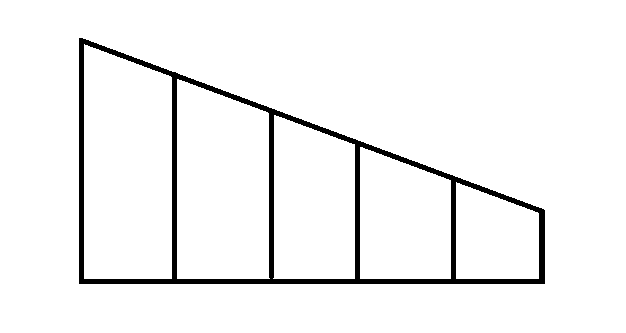
\includegraphics[width=0.7\textwidth]{images/pala dividida.png}
    \caption{Representación de una pala de turbina eólica en segmentos}
    \label{fig:pala_dividida}
\end{figure}

Por simplicidad, la pala se dividirá únicamente en $N$ segmentos, en este caso 5. Aunque se mantenga este valor durante el trabajo y es probable que no cambie, se asociará a una variable en caso de que se quieran hacer pruebas mediante MATLAB más adelante.
    
La longitud $L$ vista en la Figura \ref{fig:pala_simp} es con la que se va a trabajar, por ello cada uno de los segmentos de la Figura \ref{fig:pala_dividida} tendrá el siguiente largo $\dfrac{L}{N} = \dfrac{L}{5}$ ya que se dividió $N$ número de veces.


Como se puede observar en la Figura \ref{fig:pala_dividida} cada segmento tiene una altura variable, esto se debe a la forma real de las palas, cuanto más cerca de la turbina mayor es el tamaño del segmento.\\\\


{\color{blue} La altura de estos segmentos depende del valor de una variable, conocida como longitud de cuerda, $c$, que varía dependiendo del segmento, cuanto más alejados del rotor menor será su valor.} \\\\


\begin{definicion}
Se determina el área de los segmentos:
$$ área_{i} = \dfrac{L \cdot c_i}{N} $$
donde:
$$ i \in segmento $$
$$ segmento = \{1, ..., N\}$$
\end{definicion}

A continuación, se supone que los segmentos están separados los unos de los otros y ensartados por una línea imaginaria que ayudará al estudio de la torsión mediante giros de los segmentos alrededor suya.


\subsection{Estudio del torque con giro inicial}

El ángulo $ \theta_1 $ es la constante que se define como el giro inicial que sufrirán todos y cada uno de los segmentos que son paralelos al plano horizontal, desde el cual se presenta el viento que incidirá en nuestra pala.\\

\begin{definicion}
Dados el ángulo inicial de giro $\theta_1 $ y una variación constante de giro $\Delta_\theta$ se define el ángulo de torsión de cada segmento como:
$$\theta_i = \theta_{i-1} + \Delta_\theta$$ 

    donde:
 $$i \in segmento \wedge (i > 1)$$
\end{definicion}


Como se menciona en el primer párrafo de esta sección, el viento con el que se trabajará se presenta en el plano horizontal sobre el que también está posada la pala que estamos estudiando.\\

Al haber inclinado todos los segmentos un ángulo $ \theta_1 $ se genera la situación en la que el viento incide en el centro del segmento con el mismo ángulo con el que se inclina la pala. \\

La fuerza del viento que incide en la pala se puede descomponer en 2, la tangencial y la normal. \\

 INSERTAR DIBUJO DE LAS FUERZAS \\
 
 \begin{definicion}
 La fuerza normal genera un ángulo de:
 $$ ángulo \text{ } normal_i = \dfrac{\pi}{2} - \theta_i $$
 donde:
 $$ i \in segmento$$
 \end{definicion}

 \begin{definicion}
  Su fuerza se define como:
  $$ f \text{ } normal_i = F \cdot \sin{\theta_i}$$
   La fuerza $F$ será explicada más adelante.
  \label{def:fuerza_normal}
 \end{definicion}

 
 La componente paralela a la pala, que se ha definido como tangencial se obviará debido a que no genera momento de giro o torque. 
 
 \begin{definicion}
El momento de giro o torque se define como:
 $$ torque_i = F \text{ } perpendicular_i \times brazo_i$$
 $$ i \in segmento$$
 \label{def:torque} %para poder referenciarlo fuera
 \textcolor{red}{Brazo := distancia entre el inicio de la pala y el centro del segmento, o radio del segmento.} \\
 \end{definicion}

 La mejor forma de comprender qué se entiende por brazo es mediante la Figura \ref{fig:exp_brazo} en la cual se señalan los segmentos de la pala en distintos colores.
 
     \textbf{}
    \begin{figure}[H]
    \centering
    \includegraphics[width=1\textwidth]{images/explicación brazo.png}
    \caption{Representación gráfica del brazo de la pala}
    \label{fig:exp_brazo}
    \textit{Fuente: Elaboración propia}
\end{figure}

Ahora que visualmente se conoce qué se define por $brazo$, podemos pasar a definirlo.

\begin{definicion}
El  brazo o radio de un segmento $i$ viene definido por la siguiente fórmula:
$$ brazo_i  =  i \cdot \dfrac{L}{2 \cdot N}$$
    donde:
 $$ i \in segmento$$

\end{definicion}

 
 En la Definición \ref{def:torque} se encuentra un producto vectorial entre la $fuerza  \text{ }perpendicular \text{ } o \text{ } normal$ y el $brazo$. Pero estas dos variables son perpendiculares la una a la otra. Esto se puede ver ya que $brazo$ es completamente paralelo a la $fuerza \text{ } tangencial$. Esto demuestra la perpendicularidad y hace que la Definición \ref{def:torque} que contenía un producto vectorial de dos parámetros perpendiculares sea definitivamente un producto algebraico, dando lugar a:
 
  \begin{definicion}
  El torque termina siendo un producto vectorial.
 $$ torque_i = f \text{ } normal_i \cdot brazo_i$$
 $$ i \in segmento$$
 \label{def:torque_vectorial}
 \end{definicion}
 
\begin{definicion}
 La suma de los torques con un giro inicial se conoce como torque global.
 $$ torque \text{ } global_1 \text{ } = \sum_{i=1}^{N} torque_i $$
 donde:
 $$ i \in segmento$$
 \label{def:torque_global}
\end{definicion}

%Se ve muy pequeña la definición de toque_global
 Ahora se introduce otro concepto, se trata de la fuerza del viento. Gracias a este parámetro, podremos conocer la fuerza normal que se está produciendo en cada uno de los segmentos mediante la definición \ref{def:fuerza_normal}, ya que la fuerza $F$ es su equivalente.
 
 \begin{definicion}
 La fuerza del viento para un segmento viene definida por:
 
 $$ F \text{ } viento_i = \dfrac{1}{2} \text{ } \rho \cdot a_i \cdot u^2$$
 donde:
 
  \centering $i \in segmento$,  $\rho = 1.225 \text{ } \dfrac{Kg}{m^3}$, $a$ := área del segmento i y \\ $u$ := velocidad del viento.
 \label{def:fuerza_viento}
 \end{definicion}
 
 
 \subsubsection{Cálculo de la potencia del sistema}
 
 Una vez se tiene todo lo necesario para el cálculo del torque, se puede pasar al siguiente escalón que sería la potencia. Esta es una unidad de medida que permitirá conocer si el estudio que se está realizando está siendo fructífero, cuanta mayor cantidad de energía se genere mejor. Para conocer si la potencia que está generando el experimento se deberá realizar otro caso de estudio cambiando un pequeño parámetro que se explicará en uno de los siguientes puntos.
 
  \begin{definicion}
 La potencia del sistema con un giro inicial se define como:
 $$ potencia_1 = torque \text{ } global_1 \cdot W_1 $$ 
 
 donde:
 
 
  \centering $W_1$ := velocidad de giro o angular de las palas.
 \label{def:fuerza_viento}
 \end{definicion}
 
 